\documentclass[a4paper]{llncs}

\usepackage{amssymb}
\setcounter{tocdepth}{3}
\usepackage{graphicx}

\usepackage{url}

\usepackage{graphicx}
% \usepackage{caption}
% \usepackage{subcaption}
\usepackage[caption=false]{subfig}

\begin{document}

\mainmatter

\title{Automatic Perspective Correction of Manuscript Images}

\author{Ryan Baumann\inst{1} \and Christopher Blackwell\inst{2} \and W. Brent Seales\inst{1}}

\institute{University of Kentucky
\and
Furman University}

\maketitle

\section{Introduction}

Frequently, images of rare documents must be taken under strict time constraints, 
when a chance opportunity arises, and with equipment that is less than ideally suited 
for precise digitization. This can often result in uncalibrated images
whose contents are nonetheless qualitatively useful. Due to the logistics of document
imaging, perspective distortion is a common artifact which can manifest itself in
images taken under these constrained circumstances. We propose an automated approach for
correcting this perspective distortion, even for uncalibrated images of documents
with irregular page edges containing no regular text.

\section{Background}

In order to frame the problem and our need for a new approach, it may be helpful to first describe the images
we were working with, the circumstances under which they were taken, as well as why perspective correction was desirable.
In November of 2011, C. Blackwell and A. Hackney Blackwell photographed the botanical specimens collected in the Sloane Herbarium of the Natural History Museum, London. This was a “digitization project of opportunity”. Blackwell and Hackney Blackwell were in London working on another project, and were able to negotiate permission for this digitization at the last minute; the botanical images would complement their work on digital codicology (Blackwell) and environmental science and herbarium collections (Hackney Blackwell). The pair had one and a half working days to take as many images as possible. They had a portable conservation copystand, a tripod, and two digital cameras; the working space at the Museum was small, with limited working surfaces. The botanical specimens are pasted onto the pages of large quarto- or folio-sized volumes. An initial process of triage divided the volumes into one group that would fit on the copystand, and one group that were too large. The former were photographed with a Nikon D700 camera mounted in good alignment on the copystand, which included lightbars for even illumination. The other volumes presented a challenge.

\begin{figure}[!htbm]
  \centering

  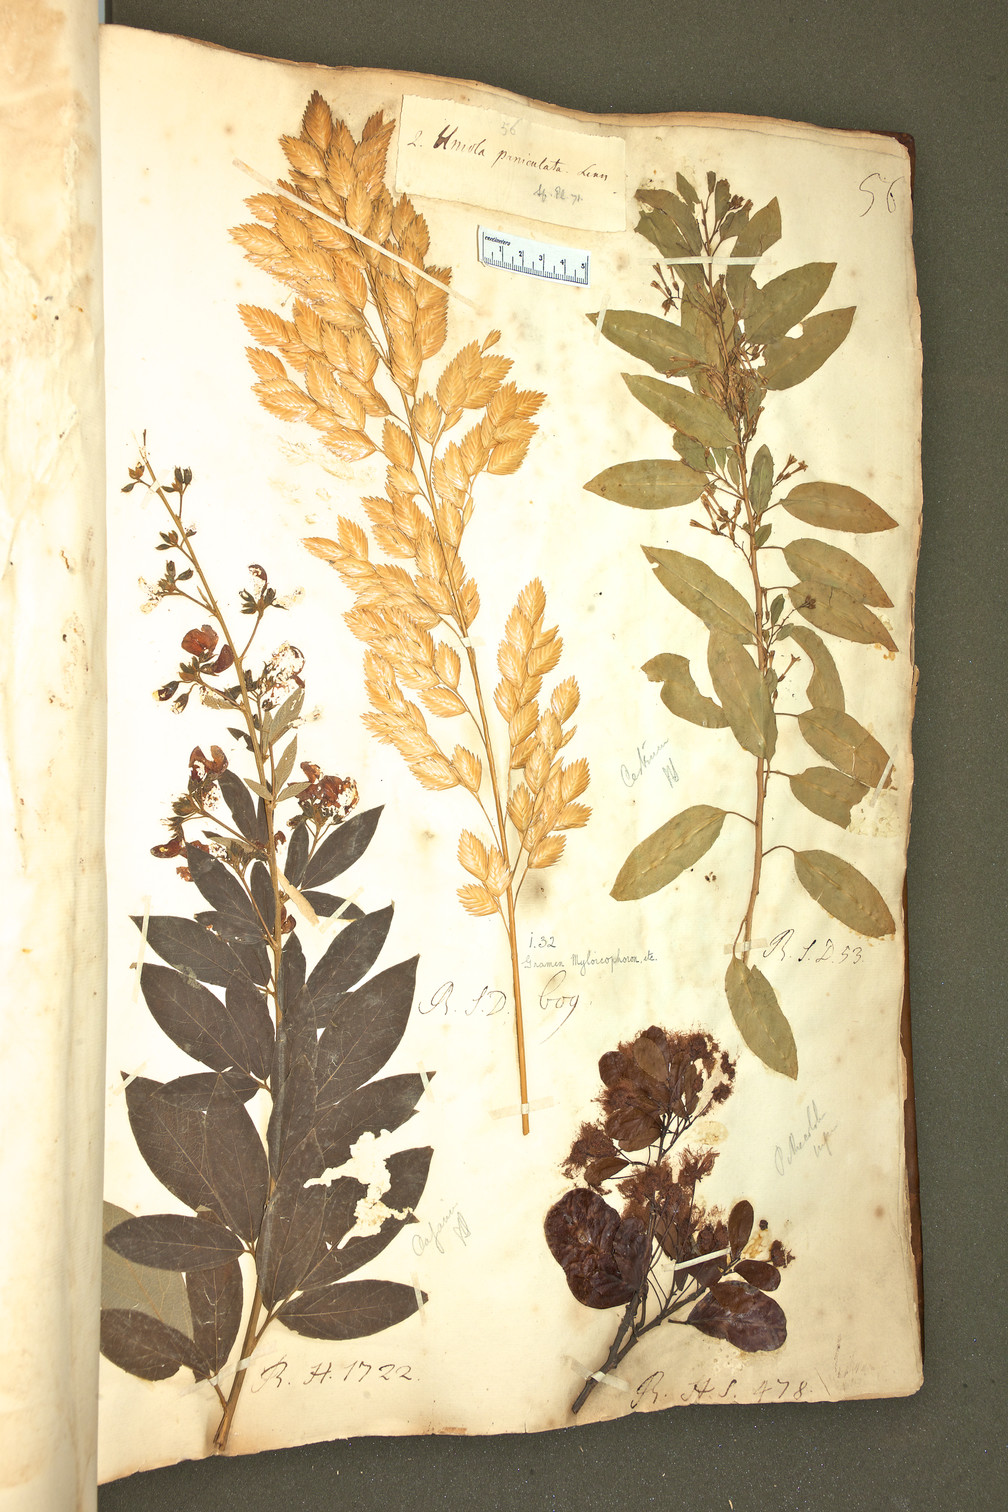
\includegraphics[height=.50\textheight]{figures/original.jpg}
  \caption{Sample original image}\label{fig:original}
\end{figure}

These were photographed with a Nikon D3x camera on a tripod; the volumes were supported by foam wedges. The tripod was weighted with exercise weights for stability, and the book, tripod, and camera were situated on an L-shaped bench. There was limited time to experiment, but the team devised an arrangement that resulted in sufficient light, good safety for the volumes being photographed, but less-than-ideal alignment of camera to page. Knowing that this alignment was imperfect, the team elected to use the camera with the higher resolution (the D3x) for these, in the hope that the greater resolution would afford greater potential for post-processing the images.

The team captured over 1,800 images in the time allotted. These books had never been photographed, and having digital access (under an Open Content License) to these 300-year-old botanical specimens is invaluable. Nevertheless, the inevitable misalignment of the images of some of the volumes is regrettable. It in no way precludes identification and study of the plant specimens, but does preclude the finest level of comparative measurement. This project resulted in a quantity of data that would not otherwise exist, but whose quality stands in need of enhancement.

\section{Related Work}

Numerous work exists for performing document perspective correction by exploiting the presence of
common text features, such as linear text baselines in printed texts
\cite{Clark:2001vj,Clark:2002wk,Clark:2003wf,Cao:2003bh,Lu:2003jy,Zhang:2005dy,Monnier:2005jj,Liang:2005hc,Ulges:2005ju,Ezaki:2005jc,Pollard:2005bp,Lu:2005ih,Avila:2005jx,Zhang:2008kj,JianLiang:2008ew,Bukhari:2009tc,Beusekom:2010dg,Luo:2011go,Rahnemoonfar:2011ux,Golpardaz:2011dz,Yang:2011dt}.
As a result, many of these techniques need to be tweaked depending upon morphological features of
the written language of the document in question.
However, for our documents,
many pages had no such features, consisting only of handwritten text and physical plant
specimens.
Other techniques use extensive calibration and data acquisition to correct for geometric distortion 
\cite{Pilu:vr,Brown:2001td,Brown:2004vl,Brown:2005uy,Brown:2007ti,LiZhang:2008bp}.
However, as detailed above, there was not sufficient time to perform this sort of data acquisition.
As a result, our approach is fairly unique in that it uses only physical page boundaries of uncalibrated images to
perform the perspective correction. An advantage to this is that it can handle “blank” pages or pages
consisting only of images or haphazard writing. In addition, because the manuscript pages we are dealing with have
cockled, uneven edges, our boundary detection needs to be relatively robust to the “noise” of these uneven edges.

\section{Perspective Correction Algorithm}

The perspective correction algorithm functions by applying a few steps in sequence:

\begin{figure}[htbm]
  \centering

  \subfloat[Masked image]{
    
\includegraphics[width=.48\textwidth]{figures/Catesby_HS232_056_0602-masked.jpg}
    \label{fig:masked}
  }
  \subfloat[Canny edge lines]{
    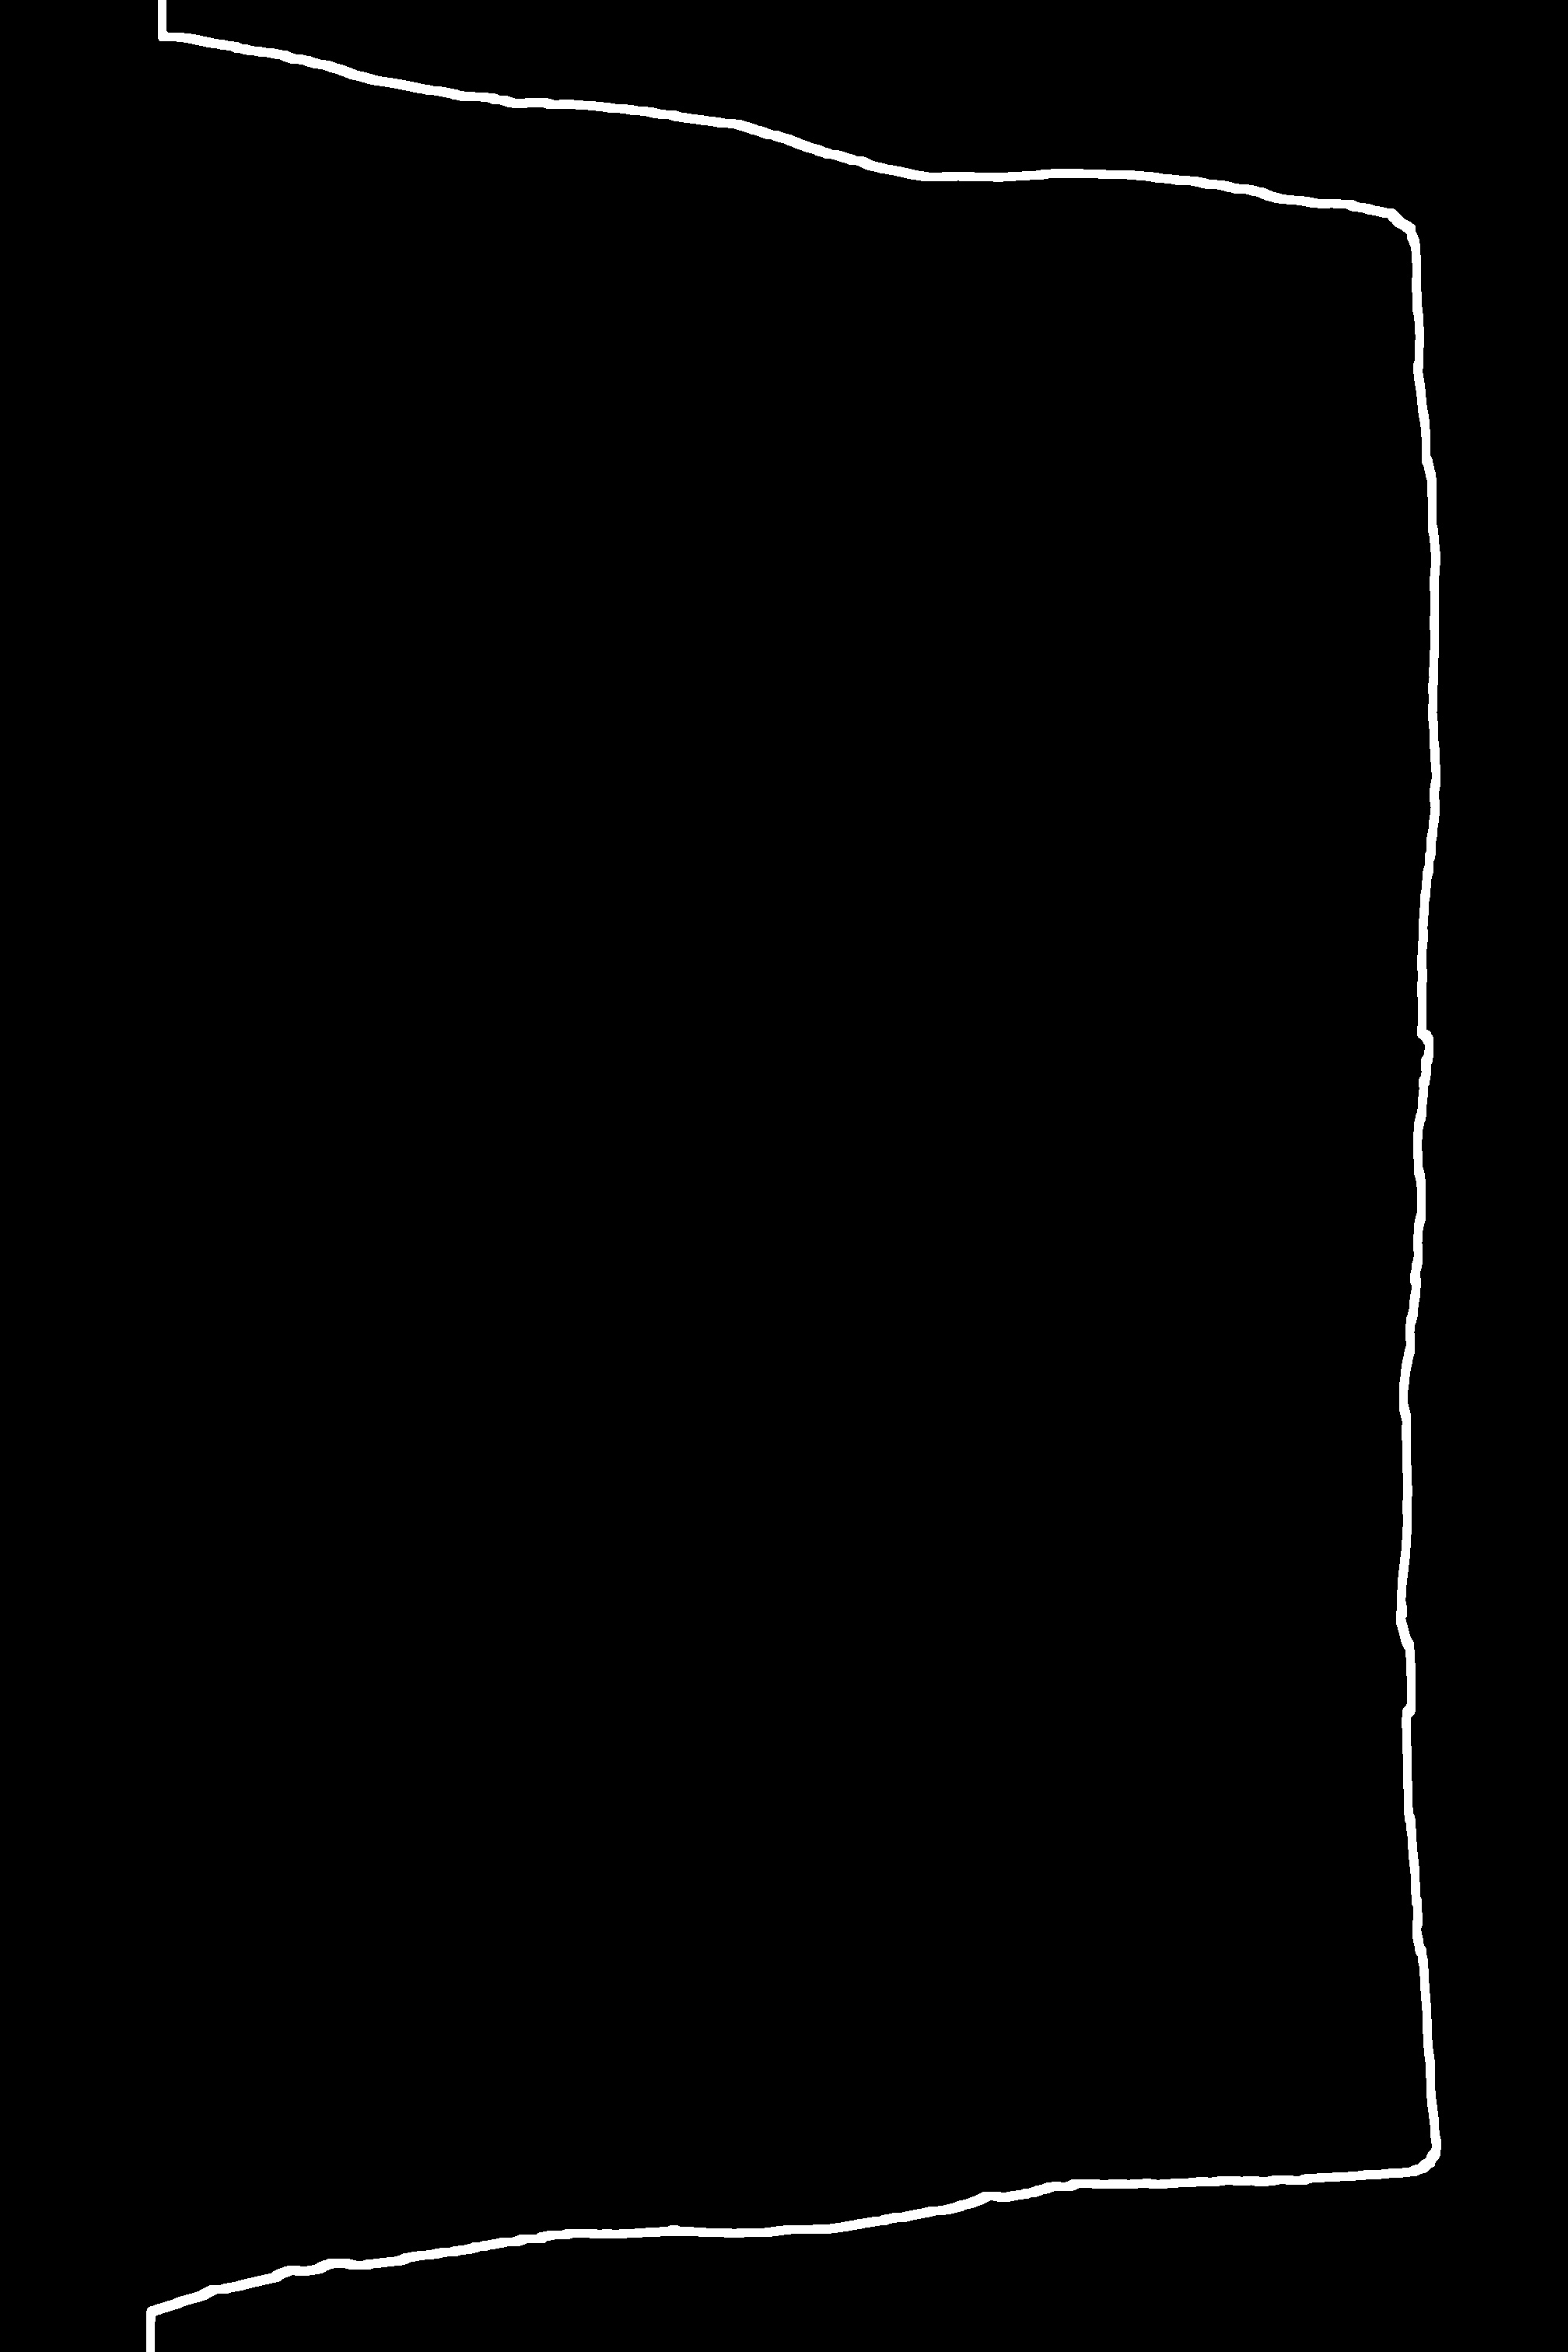
\includegraphics[width=.48\textwidth]{figures/Catesby_HS232_056_0602-canny.jpg}
    \label{fig:canny}
  }

  \subfloat[Hough line detection]{
    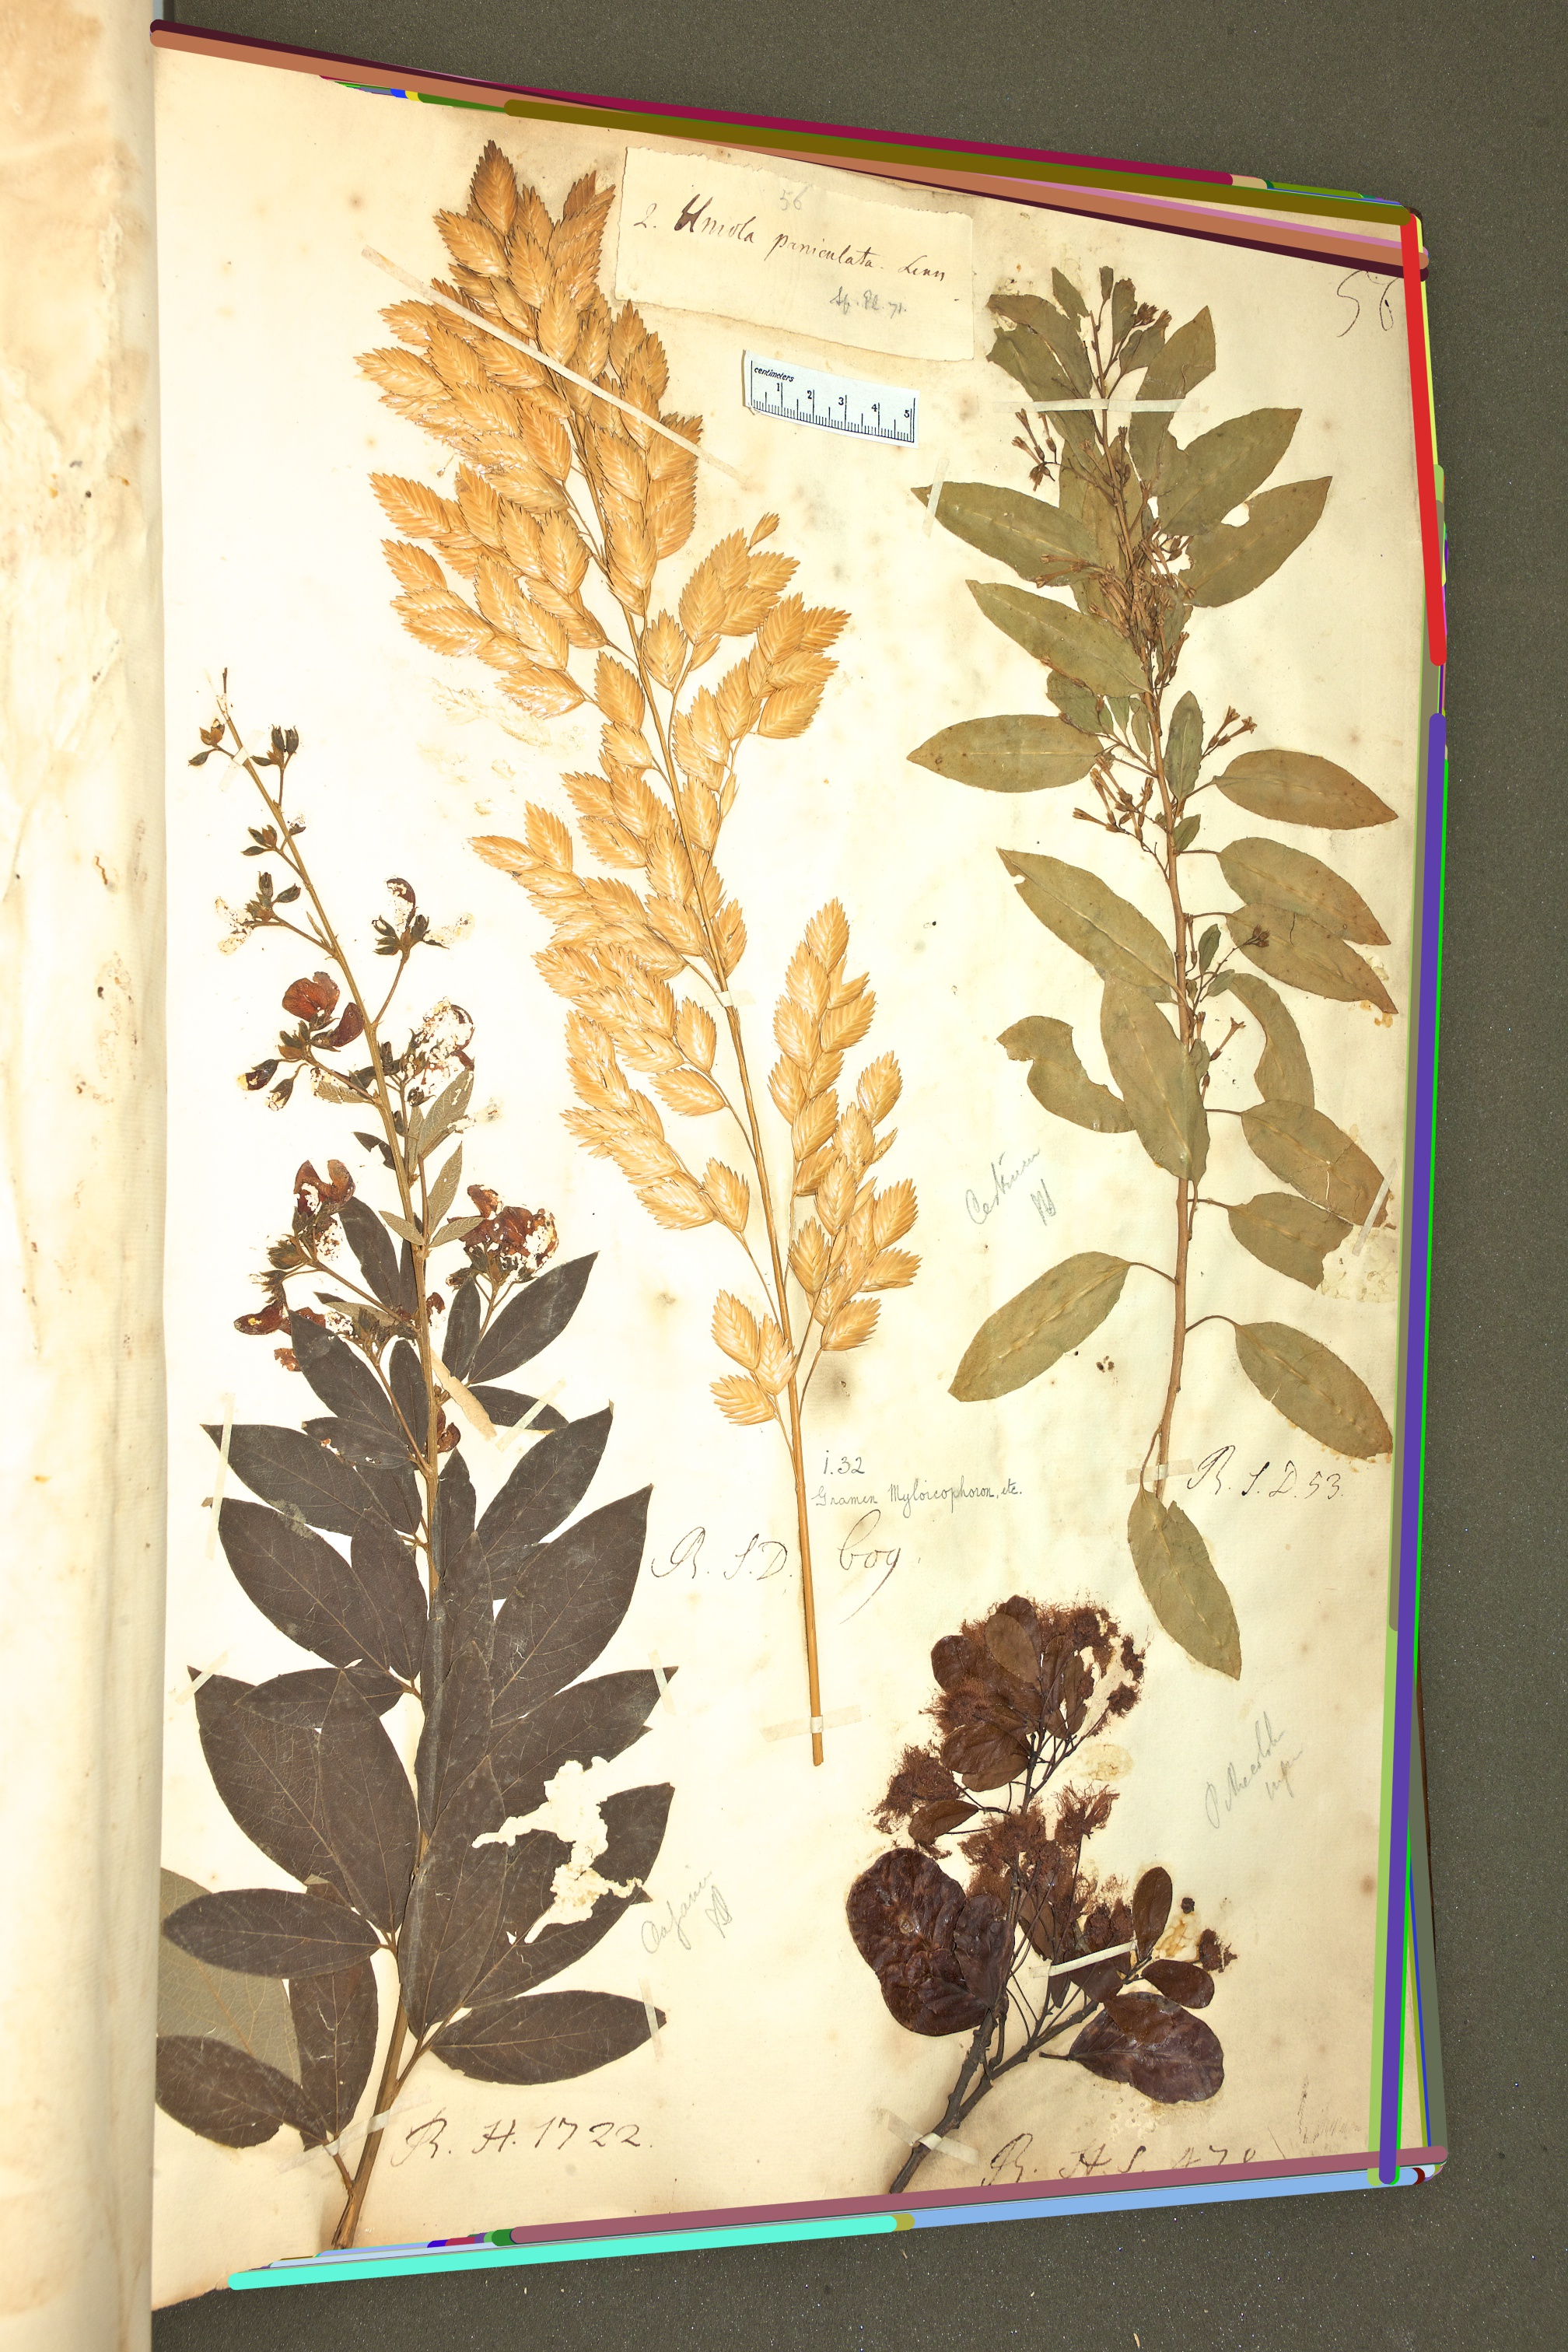
\includegraphics[width=.48\textwidth]{figures/Catesby_HS232_056_0602-hough.jpg}
    \label{fig:hough}
  }
  \subfloat[Classified lines]{
    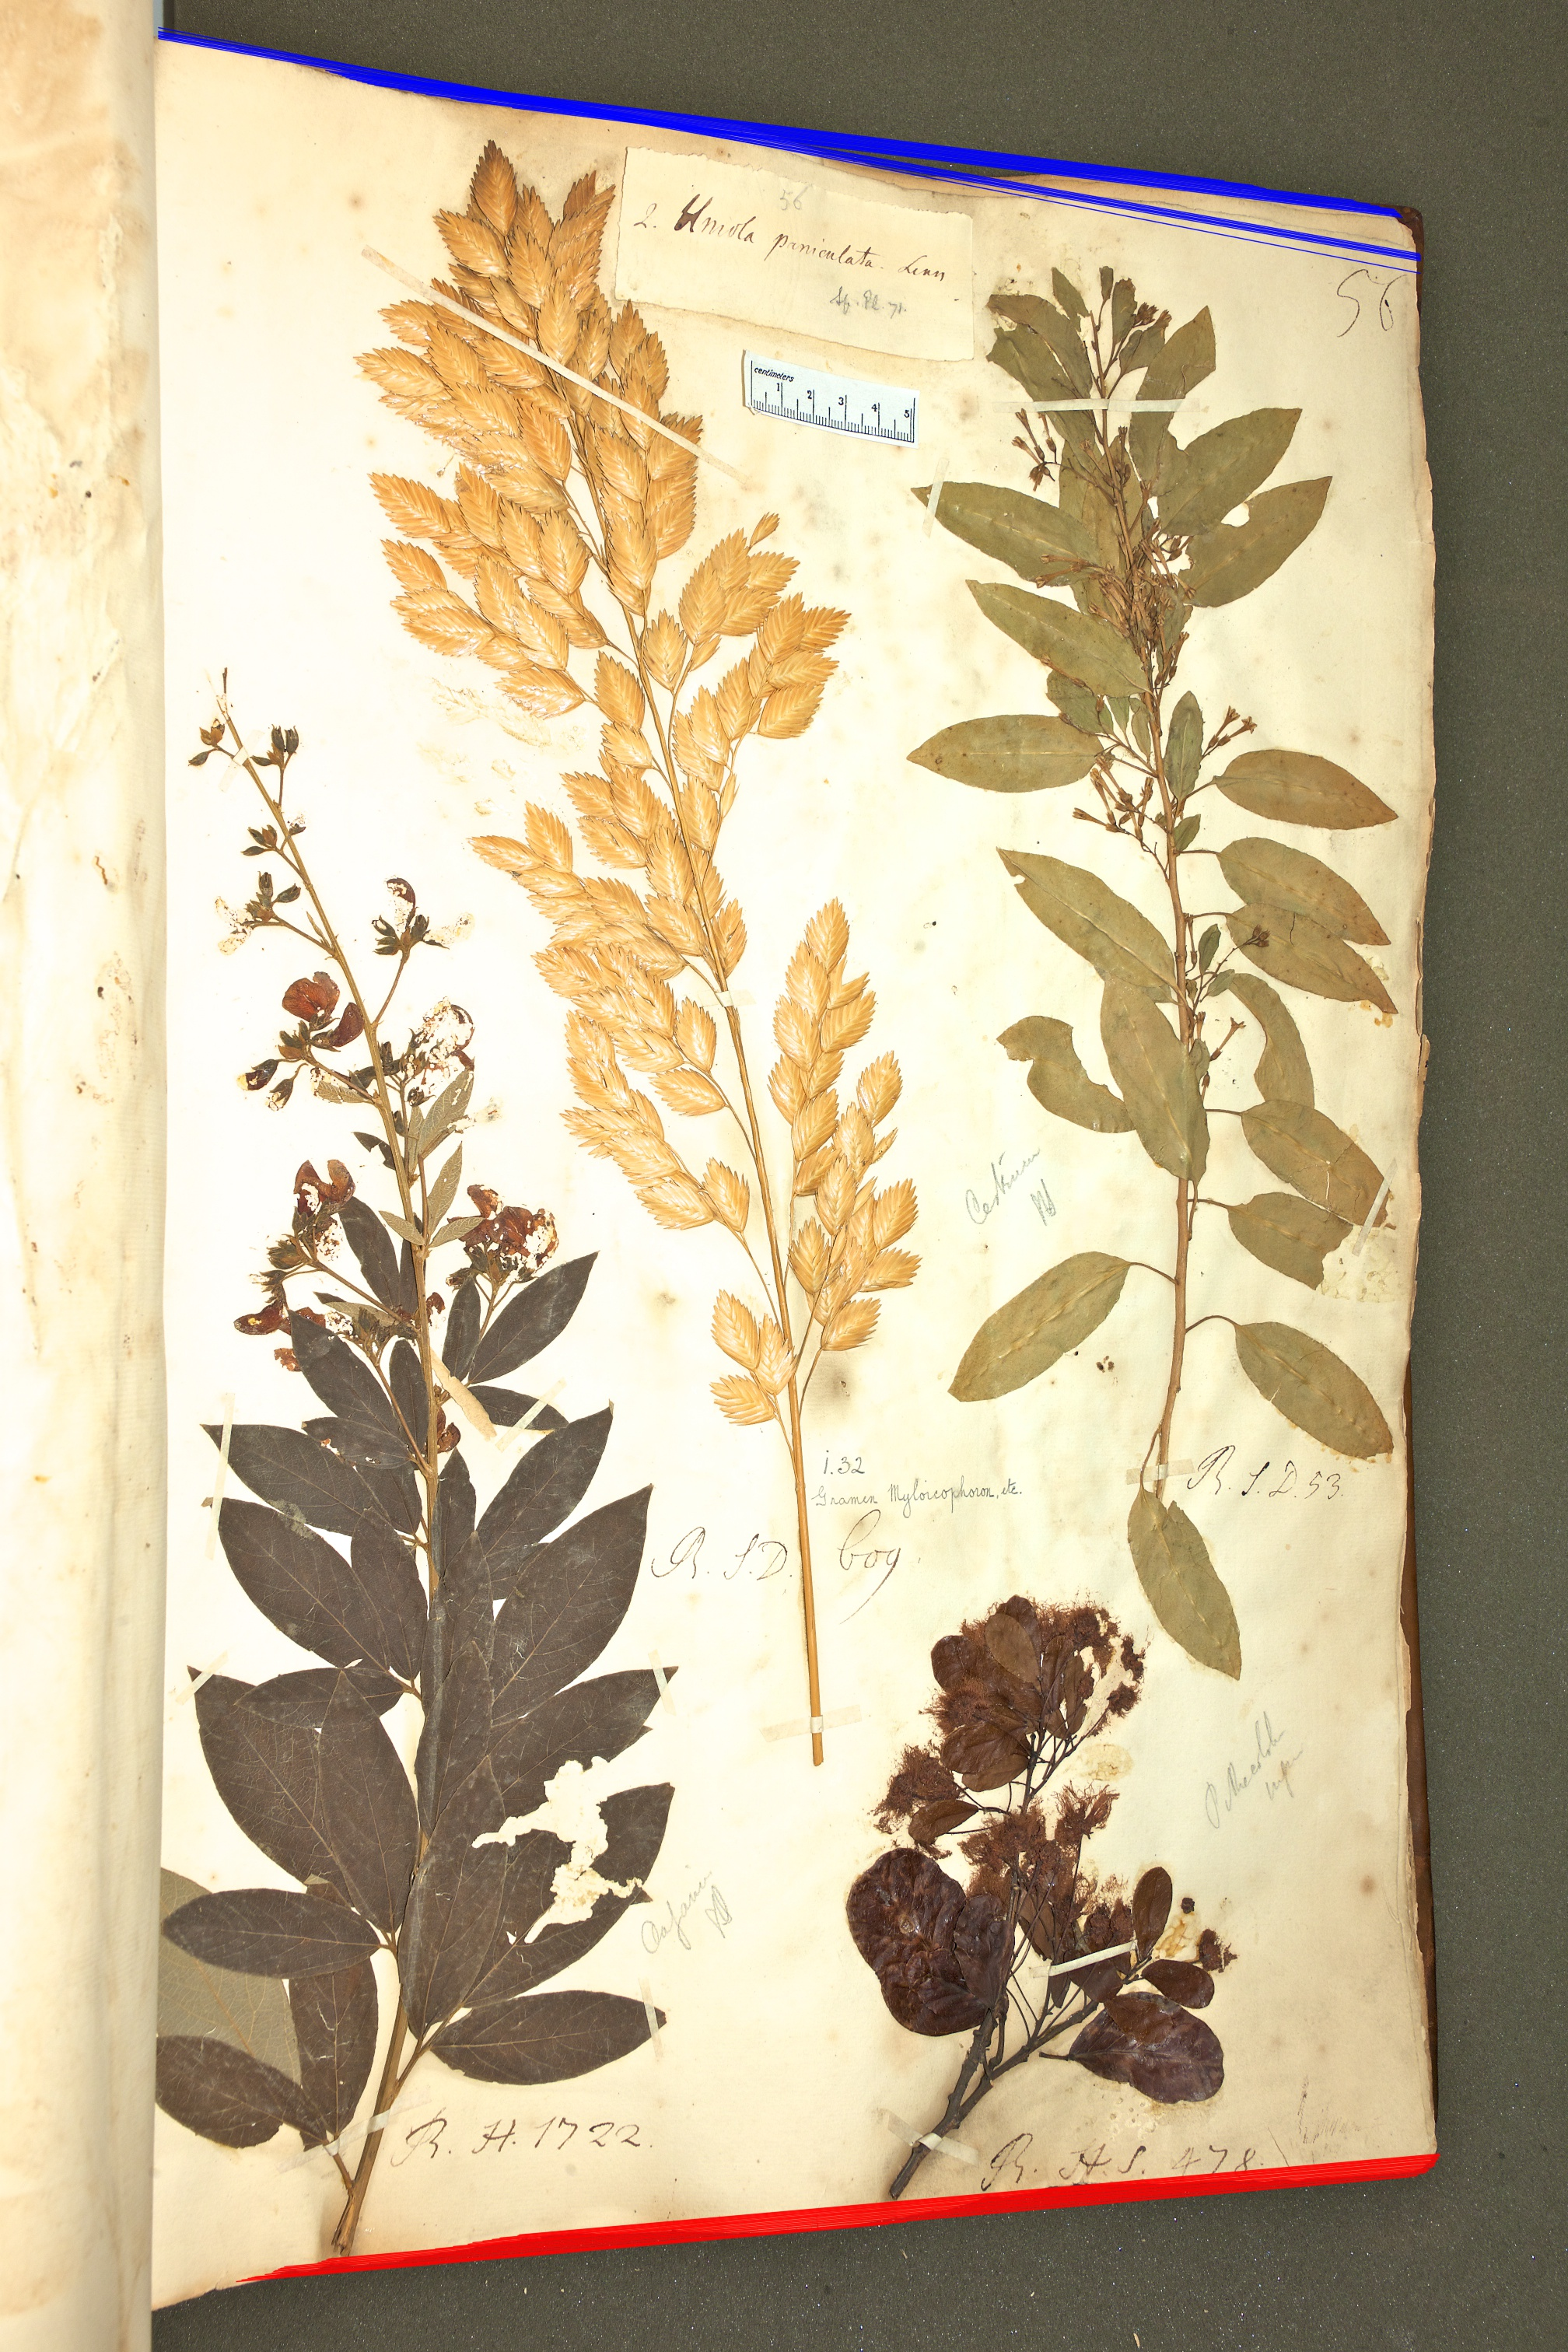
\includegraphics[width=.48\textwidth]{figures/Catesby_HS232_056_0602-hough-classified.jpg}
    \label{fig:classified}
  }
  \caption{Pre-processing steps}\label{fig:processing}
\end{figure}

\begin{figure}[htbm]
  \centering

  \subfloat[Averaged lines]{
  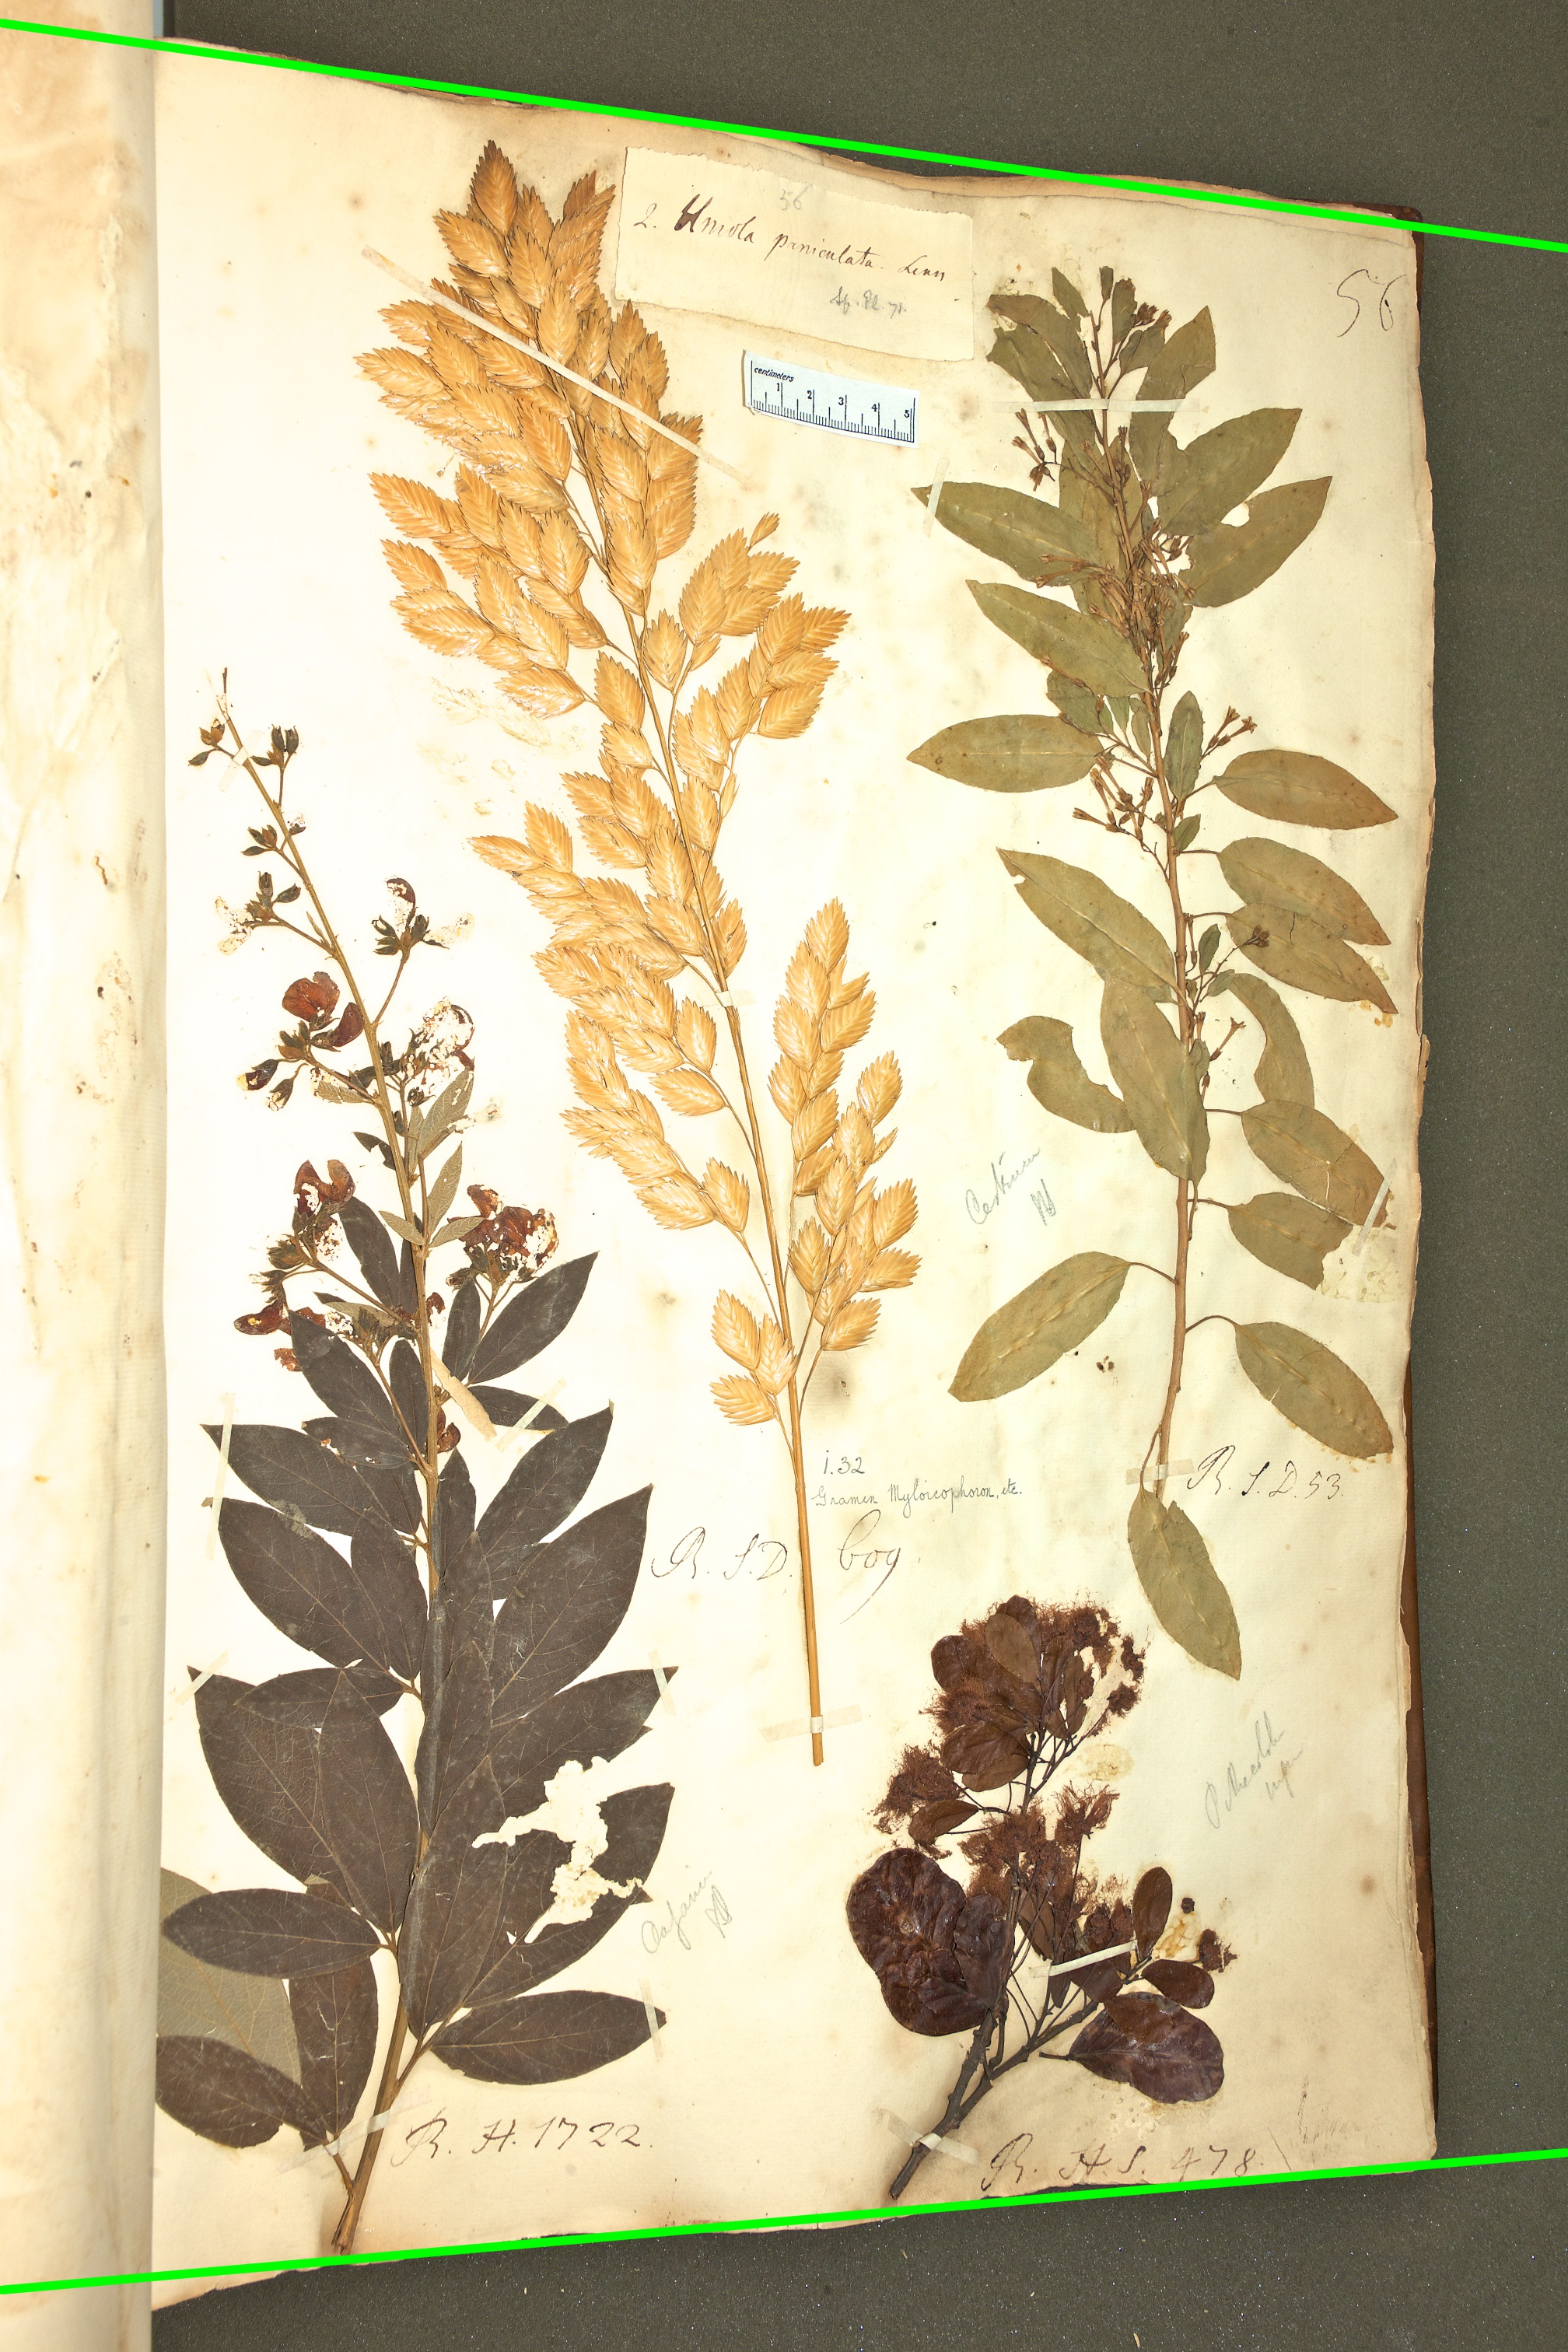
\includegraphics[height=.35\textheight]{figures/Catesby_HS232_056_0602-hough-averaged.jpg}
  \label{fig:averaged}
  }
  \subfloat[Unwarped image]{
  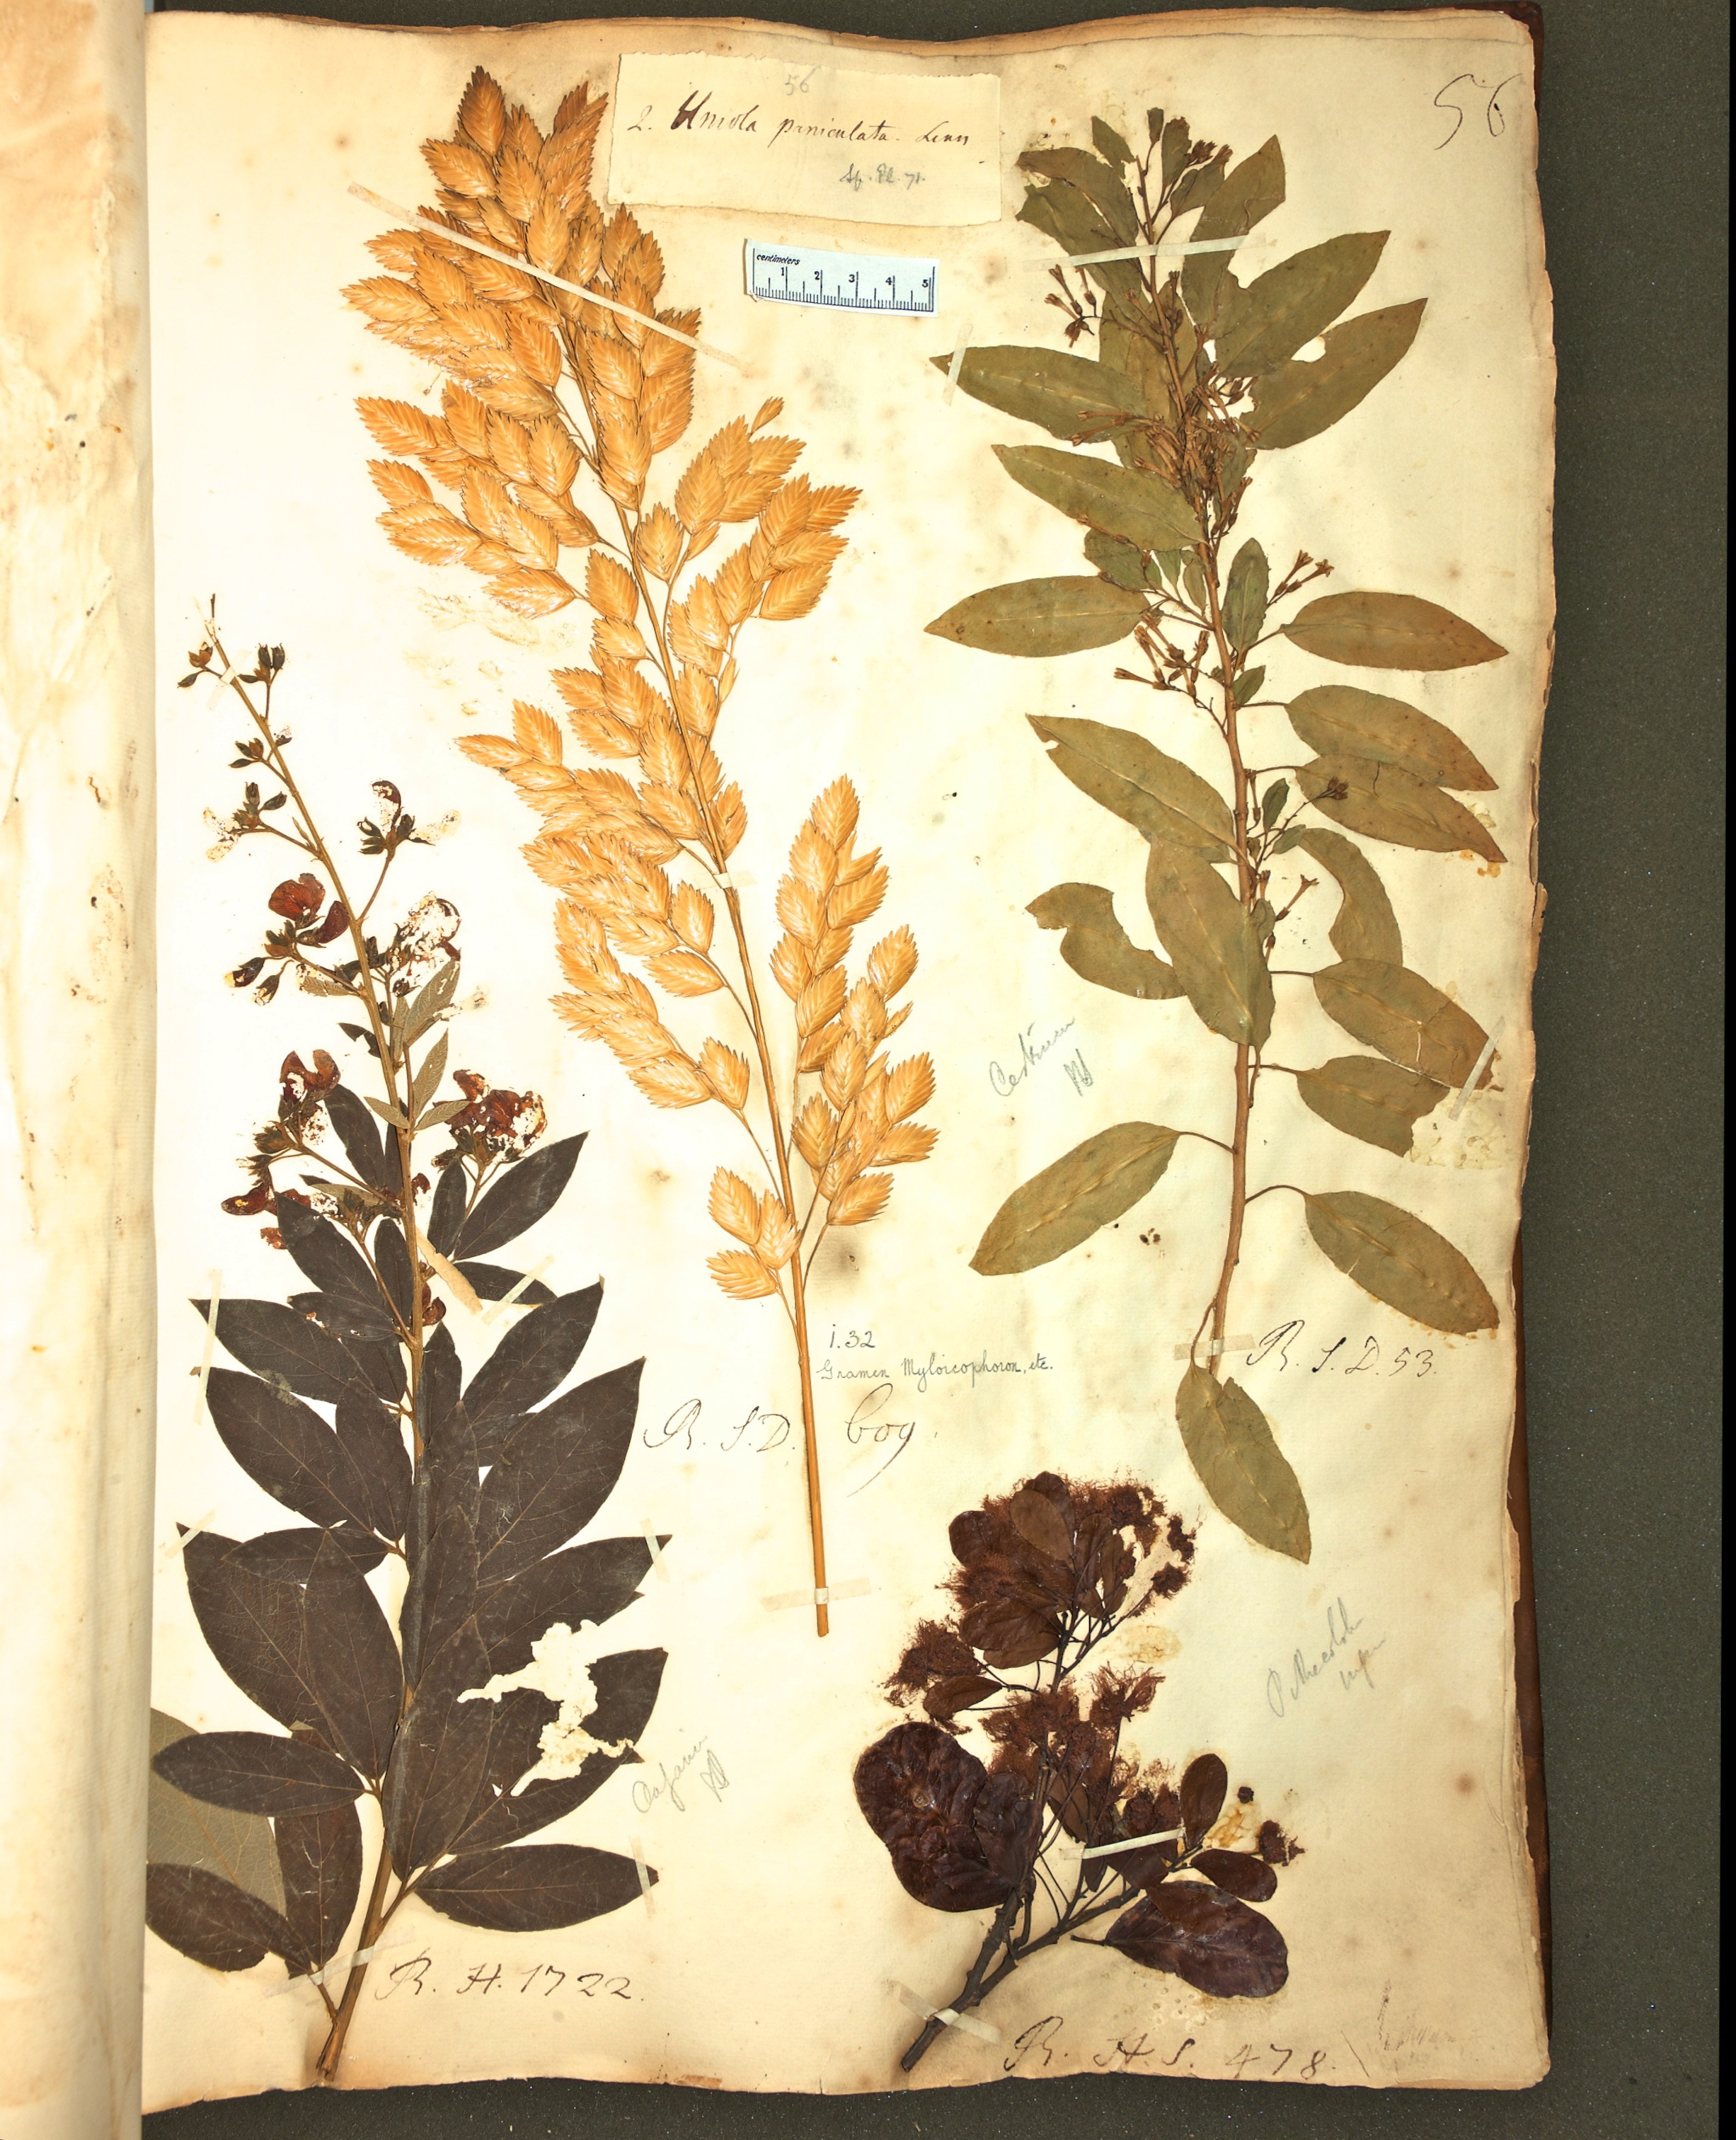
\includegraphics[height=.35\textheight]{figures/Catesby_HS232_056_0602-unwarped-stretch.jpg}
  \label{fig:unwarped}
  }
  \caption{Final perspective processing}\label{fig:final}
\end{figure}

\begin{figure}[htbm]
  
\end{figure}

\begin{enumerate}
  \item Foreground/background segmentation. (Figure \ref{fig:masked})
  \item Canny edge detection followed by dilation to turn the mask image into a line image. (Figure \ref{fig:canny})
  \item Hough line detection to detect lines. (Figure \ref{fig:hough})
  \item Line classification to classify the detected lines as “top” or “bottom” page edge lines. (Figure \ref{fig:classified})
  \item Line averaging to find the “average” line for the top and bottom edge lines. (Figure \ref{fig:averaged})
  \item Compute homography for transforming the slanted top and bottom page lines into straight lines.
  \item Application of the resulting perspective warp. (Figure \ref{fig:unwarped})
\end{enumerate}

For our images, most were made with a fairly consistent backdrop, so the foreground/background segmentation operates by performing a flood fill on the corners of a gaussian-smoothed version of the image. This exploits the assumption that the page will not fill the full image all the way around, as in such a case, our perspective correction would likely be unable to accurately detect all the page edges which it uses to compute homography. We then remove blobs whose area is less then half the image, as we assume the page still makes up most of the image. 

This gives us a mask image as seen in Figure \ref{fig:masked}. Since we want to use Hough line detection, we first need to transform the mask edges into lines, which we do using a Canny edge detector and dilation, the results of which can be seen in Figure \ref{fig:canny}.

We can then perform Hough line detection, using a probabilistic Hough transform which gives us line segments for every line detected in the image. We classify these lines as belonging to either the “top” or “bottom” of the page by seeing which half of the image height the start and end points are in, and restricting it to only lines with a $\pm 45\,^{\circ}$ angle. This also filters out edges detected along the left and right side of the page.

We can then average these lines to get the average “line” for the top and bottom page edges. We extend these lines to the image edges, and construct a quadrilateral matrix using them for the top and bottom. We then compute a destination quadrilateral matrix using the assumption that the top edge should be “brought up” to the highest point to form a straight line (while maintaining line length), and similarly for the bottom edge being brought down, forming a rectangle. We can then use these two quads to compute a perspective transform which will warp our source quadrilateral into our destination rectangle. We then apply the resulting perspective warp to the whole image, resulting in a dewarped image, as seen in Figure \ref{fig:unwarped}.

Because the process currently operates with no knowledge of the camera field of view or focal length parameters,
the aspect ratio of the final dewarped image must still be corrected. This is because although we can bring the
edges parallel, we do not know their actual physical depth and the resulting scale needed in one direction,
which will be affected by the camera field of view. This can be corrected using \emph{a priori} knowledge of the
document's aspect ratio, or in our case we have a small ruler in the image on the page
which we can use after perspective correction to correct the aspect ratio.

\section{Results}

In processing the hundreds of herbarium images which required perspective correction, almost all succeeded
with no need for manual intervention. Occasionally, an image with some discontinuous feature in the background
would fail the foreground/background segmentation step, but this is fairly easy to correct with some minor
image pre-processing. In any case, the perspective correction enables much more accurate comparative measurements
to be made on the specimens contained in our page images.

\begin{figure}[h!tbm]
  \centering

  \subfloat[Before perspective correction]{
    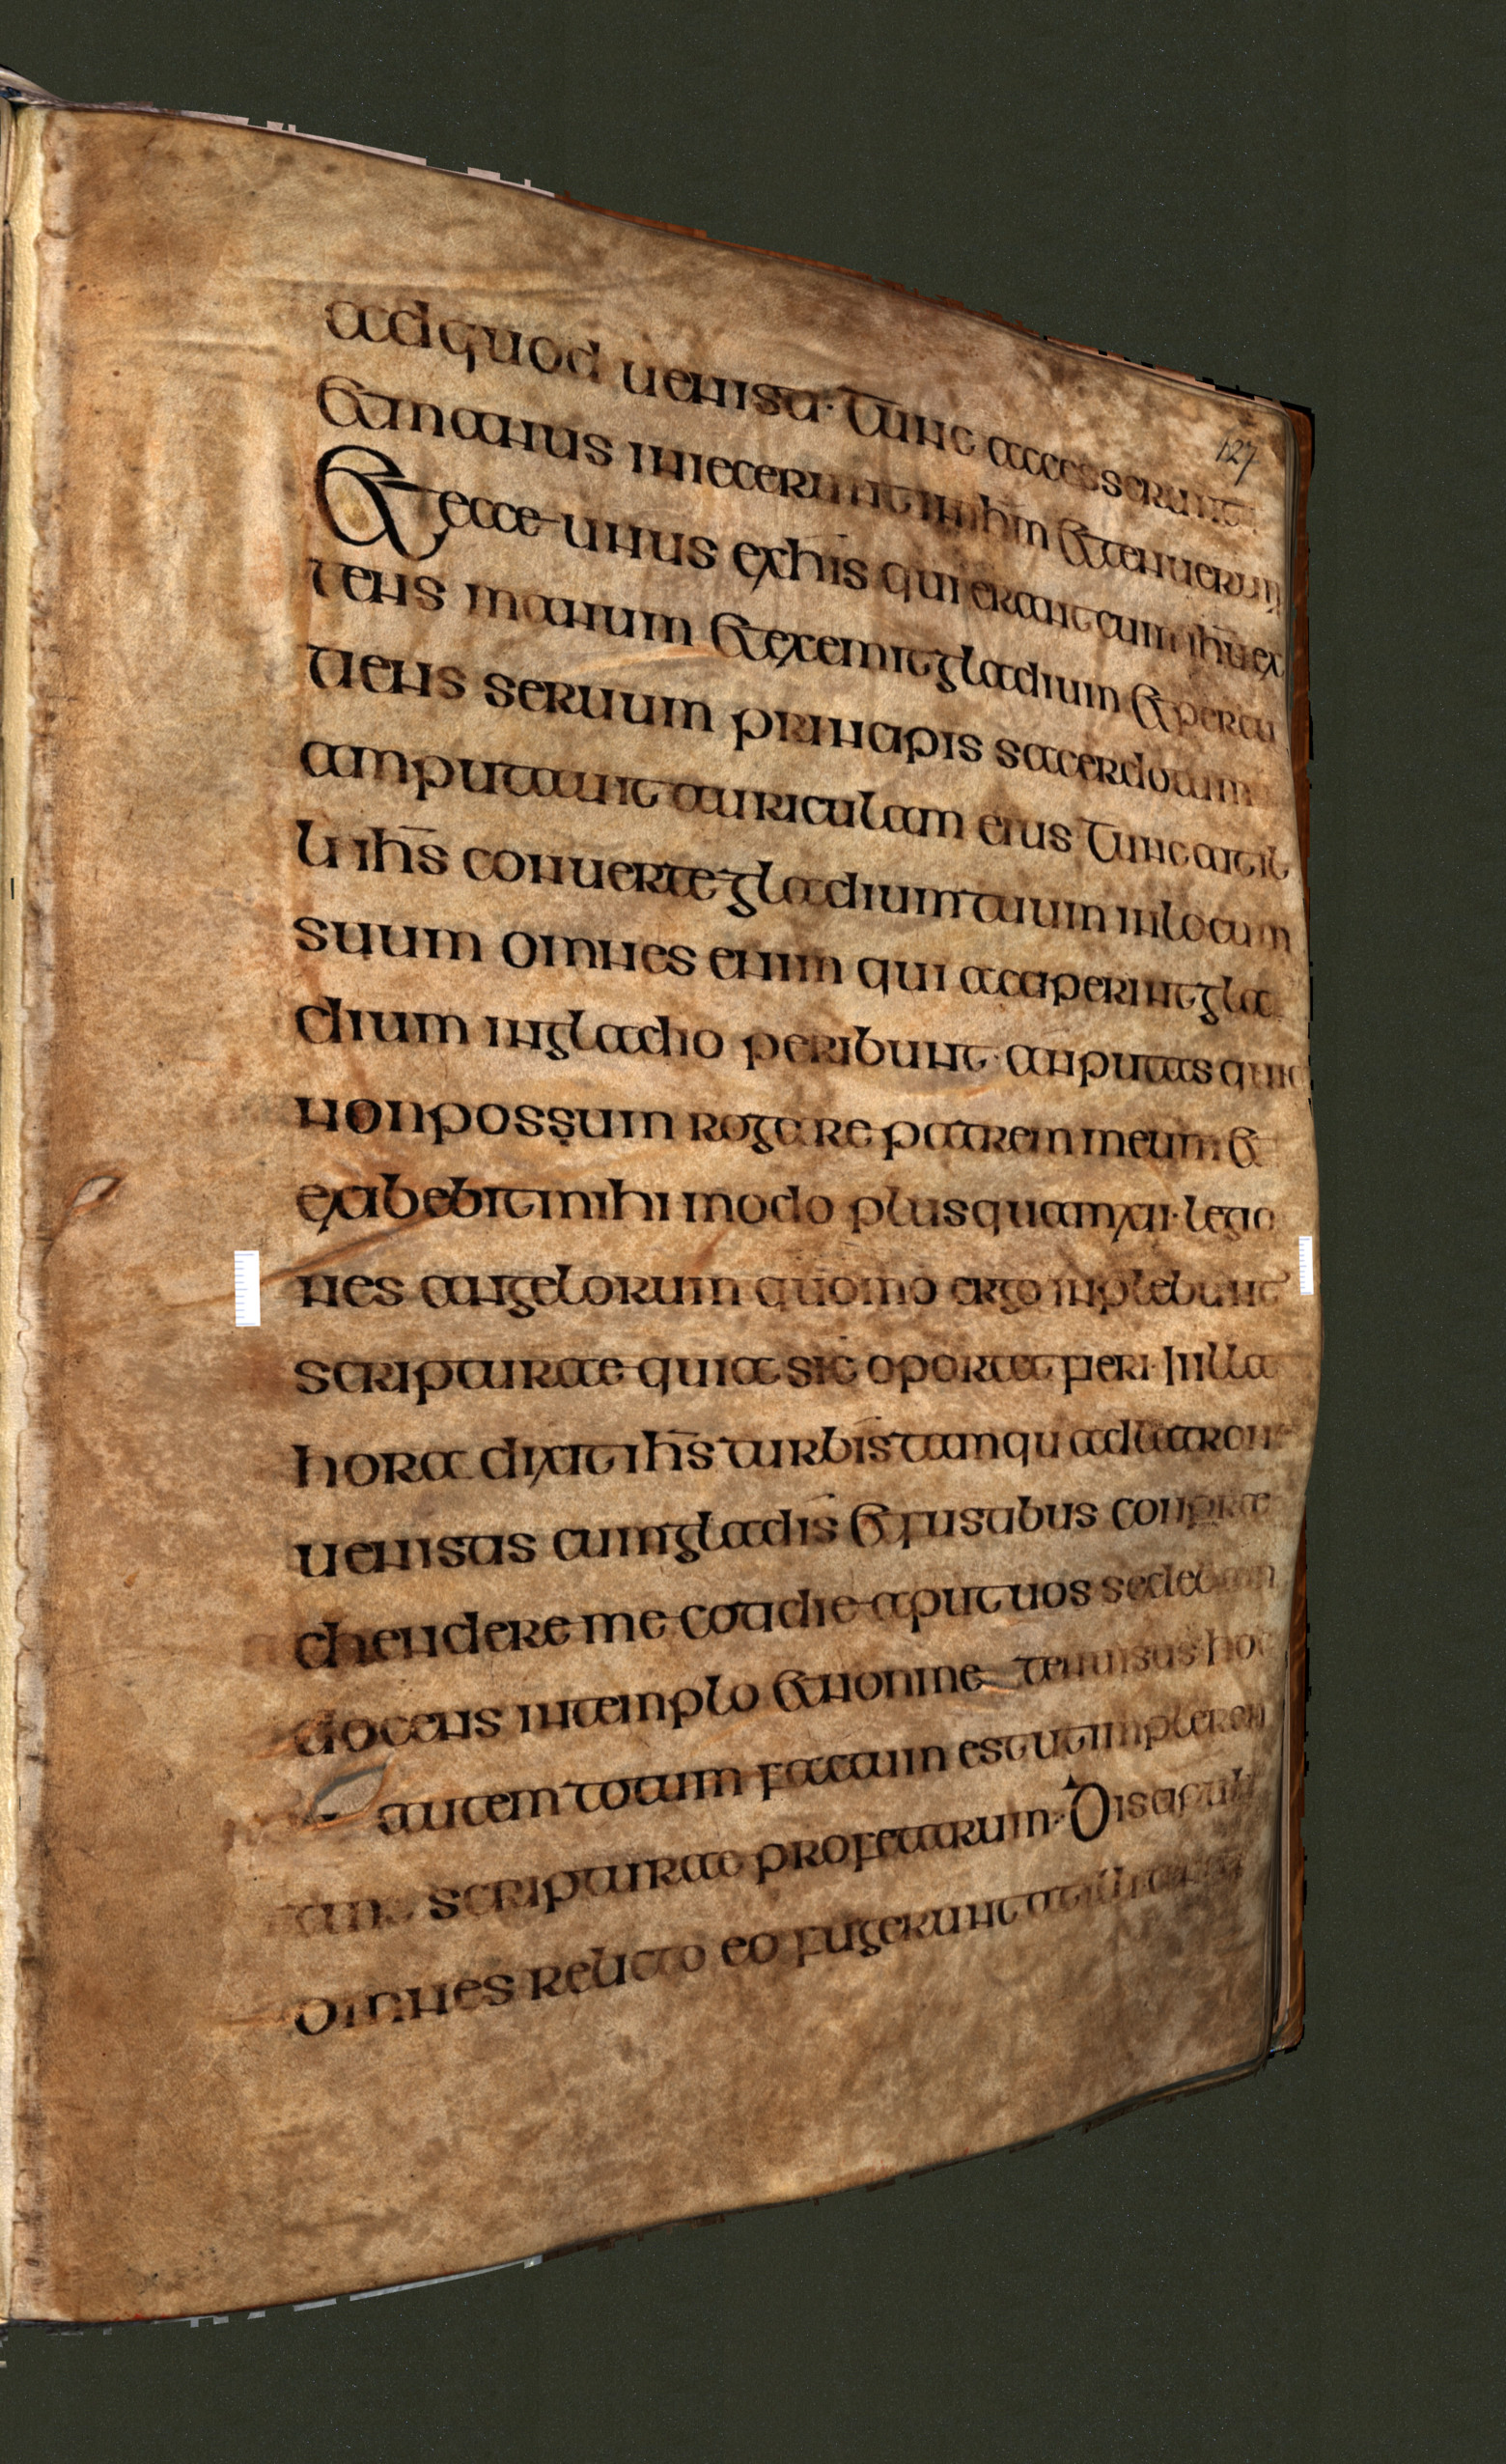
\includegraphics[height=.35\textheight]{figures/snapshot-fiducial-withbg.png}
    \label{fig:synthetic-before}
  }
  \subfloat[After perspective correction]{
    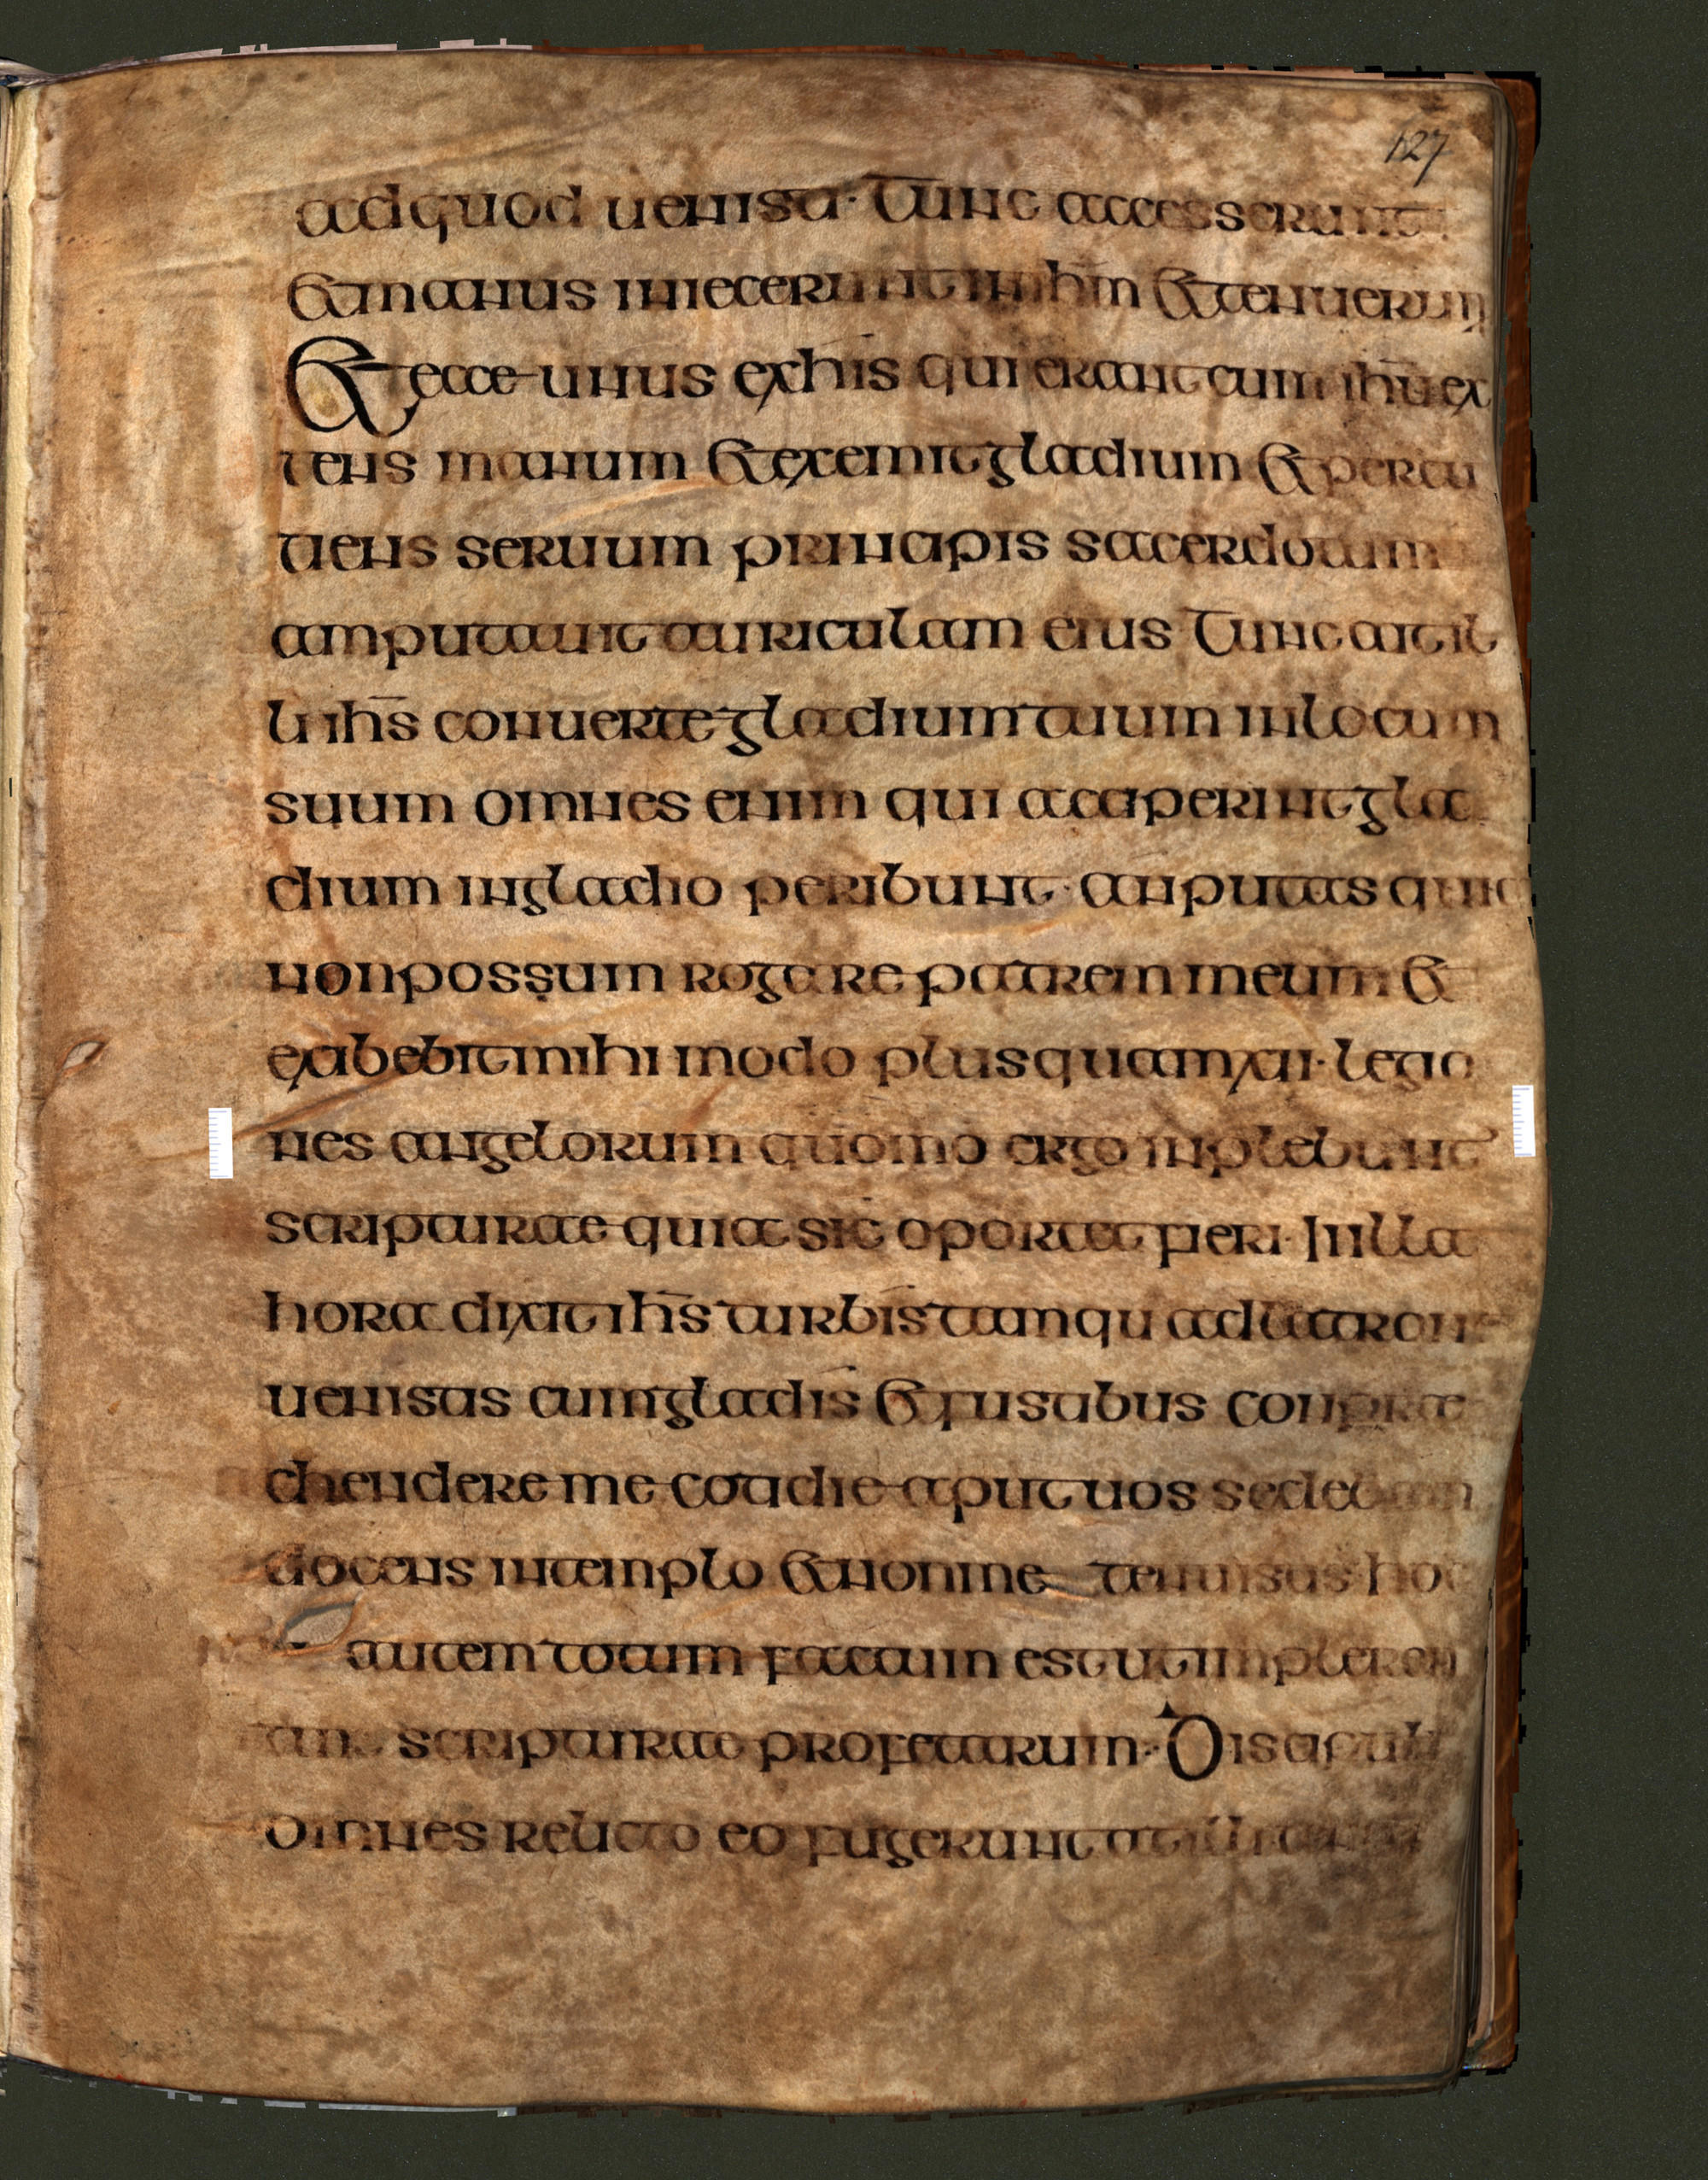
\includegraphics[height=.35\textheight]{figures/snapshot-fiducial-withbg-unwarped-ar.jpg}
    \label{fig:synthetic-after}
  }
  
  \caption{Verifying system accuracy with synthetic page images rendered using 3D scan data. The white fiducial markers can be seen on the left and right margins of the page.}\label{fig:synthetic}
\end{figure}

In order to verify the system, we also applied it using control 3D manuscript image data we had previously acquired.
In this case, we had accurate, metrically calibrated, 3D surfaces and corresponding texture data for an ancient manuscript. By placing synthetic 1cm measurement fiducials on the surface and rendering it in a scene with perspective distortion,
we can then in turn apply our automated perspective correction algorithm to the rendered image to verify its accuracy. For the image shown in Figure \ref{fig:synthetic}, the 1cm fiducials are 144px and 111px before correction, and both measure 153px after correction.

\section{Conclusions and Future Work}

The method described here is relatively robust and fast to perform on a large number of high-resolution images.
For different images where assumptions exploited by this method might not hold, for example in 
foreground/background segmentation, a different approach or altered parameters
may need to be used for a particular step.

Future work could be done in automating the aspect ratio correction after perspective correction. We plan to
investigate if camera metadata is sufficient for using focal length and field of view parameters to perform this
correction automatically, or performing a first pass for refinement.

\section{Acknowledgments}

We would like to thank the Natural History Museum, London for permission and access in imaging items from their collection. We would also like to thank the Chapter of Lichfield Cathedral for their permission in imaging the Chad gospels,
which are used for the synthetic image results and distributed under a Creative Commons Attribution-NonCommercial-ShareAlike 3.0 Unported License.
%We would also like to thank (other thanks go here).

This material is based in part upon work supported by the National Science Foundation under Grant Numbers
IIS-0916421 (other grants go here).
Any opinions, findings, and conclusions or recommendations expressed in this material are those of the authors
and do not necessarily reflect the views of the National Science Foundation.

\bibliographystyle{splncs}
\bibliography{icadl12}

\end{document}
